\documentclass[border=20pt]{standalone}
\renewcommand\familydefault{\sfdefault} % Default family: serif 
\usepackage[usenames,dvipsnames]{xcolor}
\usepackage{tikz}
\usepackage{soul}
\usetikzlibrary{calc} 
\usetikzlibrary{arrows, decorations.markings,positioning,backgrounds,shapes}
\definecolor{WIRE}{HTML}{002FA7} % Klein Blue
\usepackage{ulem}
\renewcommand{\ULdepth}{3pt}

\newcommand\whiteuline{\bgroup\markoverwith
	{\textcolor{white}{\rule[-0.5ex]{2pt}{0.4pt}}}\ULon}

\tikzset{FK/.style={thick,<-,thick,>=latex}}

\newbox\ubox
\begin{document}
	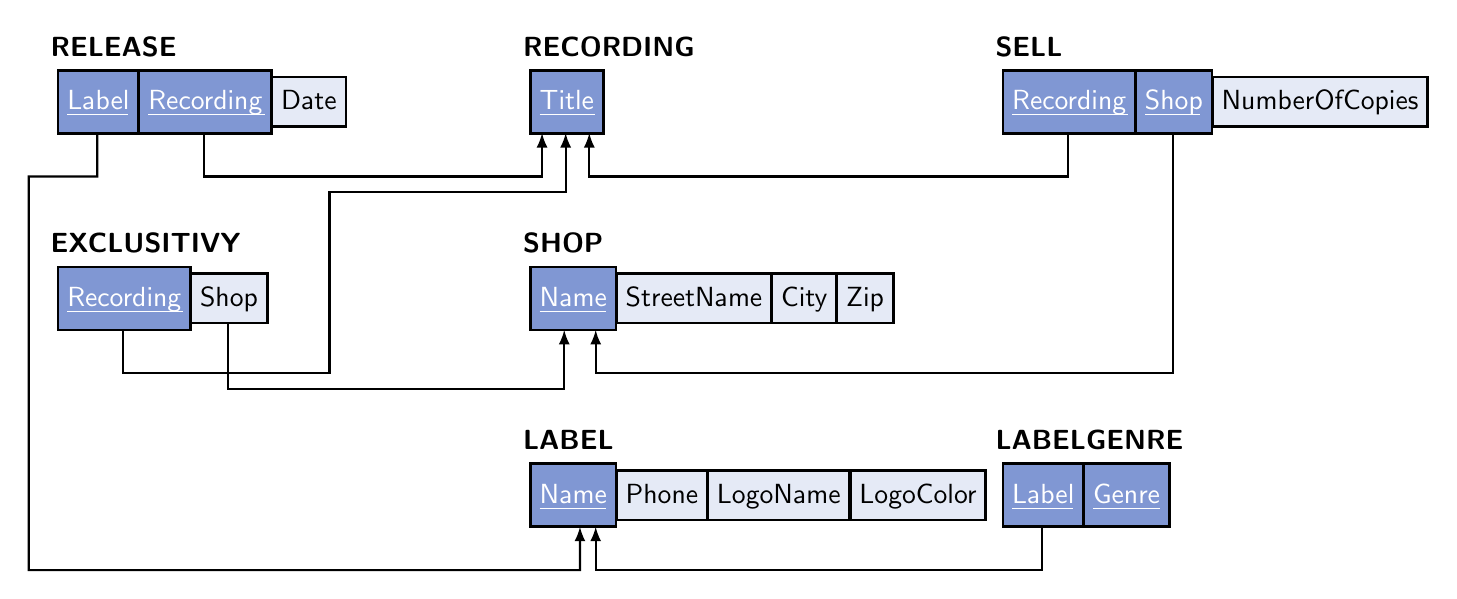
\begin{tikzpicture}[
	PK/.style={% Style for empatized boxes
		rectangle, line width =1pt,
		anchor=west,
		underline, % new property
		align=center,
        text=white,
		minimum height=.8cm,
		text height=1.5ex,
		text depth=.25ex,
        fill=WIRE!50,
		draw=black,
	},
	A/.style={% Style for normal boxes.
		rectangle, 
		line width =1pt,
		anchor=west,
		align=left,
		minimum height=.6cm,
		text height=1.5ex,
		text depth=.25ex,
        fill=WIRE!10,
		draw=black,
		inner ysep=5pt
	},
	underline/.append style={% define new style property
		execute at begin node={%
			\setbox\ubox=\hbox\bgroup
		},
		execute at end node={%
			\egroup\whiteuline{\box\ubox}%
		}
	},
	] % Uff that is all the configuration for tickzpicture xD
	
	% Define an brute force objet "Frame"
	% Variables 1:Position, 2: Identifier, 3: Title of frame 4: Subframe/Boxtype
	\def\Frame(#1)#2[#3]#4{%
		\begin{scope}[shift={(#1)}] 
		\node[font=\bf, anchor=west] (Title) at (-0.2,0.7) {#3}; 
		\edef\k{0}% Variable for box positión
		\edef\x{0}% Variable for named coordinate centering - below box
		\foreach \id/\style in {#4} {%enter sub frame data Name/Boxtype ,Name2/Boxtype | An space before Boxtype is needed 
			\node[\style] (h) at (\k pt,0) {\id}; %  % Draw a node depending on the variables.
			\pgfmathparse{\k+0.5*width{"\id"}+3.4pt} % Uses the textwidth to calculate named coordinate  
			\xdef\x{\pgfmathresult} % The resul is saved in the variable \x
			\draw (\x pt,-0.4) coordinate (\id#2); %Create a named coordinate concatenated: "sub frame data Name"+"identifier"
			\pgfmathparse{\k+width{"\id"}+6.8pt}% Calculate positión for each subframe box.       
			\xdef\k{\pgfmathresult}% Save the value to be added to the next iteration value.
		}    
		\end{scope}
	}% disadvantages: Is not posible to use Frame data Name like: Name_another_desc instead I use Name-another-desc


% RELEASED(Label (PK, FK to LABEL.Name), Recording (PK, FK to RECORDING.Title), Date)
% EXCLUSITIVY(Recording (PK, FK to RECORDING.Title), Shop (FK to SHOP.Name))
% RECORDING(Name (PK))
% SHOP(Name (PK), StreetName, Citiy, Zip)
% LABEL(Name (PK), Phone, LogoName, LogoColor)
% SELL(Recording (FK, PK to RECORDING.Title), Shop (PK, FK to SHOP.Name), NumberOfCopies)
% LABELGENRE(Label (PK, FK to LABEL.Name), Genre (PK))

\Frame(0,0){1}[RELEASE]{
	Label/PK,
	Recording/PK,
	Date/A};

\Frame(0,-2.5){2}[EXCLUSITIVY]{
	Recording/PK,
	Shop/A};

\Frame(6,0){3}[RECORDING]{
	Title/PK};

\Frame(6,-2.5){4}[SHOP]{
	Name/PK,
	StreetName/A,
	City/A,
	Zip/A};

\Frame(6,-5){5}[LABEL]{
	Name/PK,
	Phone/A,
	LogoName/A,
	LogoColor/A};

\Frame(12,0){6}[SELL]{
	Recording/PK,
	Shop/PK,
	NumberOfCopies/A};


\Frame(12,-5){7}[LABELGENRE]{
	Label/PK,
	Genre/PK};

\draw[FK] % From Label1 to Name3⁵
(Name5)++(0.1,0) -- ++(0,-.55) -- ++(-7,0) 
 -- ++(0,5) coordinate (inter)
 -- ++(0.87,0) coordinate (inter)
 -- (Label1);
 
\draw[FK] % From Recording1 to Title3
(Title3)++(-0.3,0) -- ++(0,-.55) coordinate (inter)
-- (Recording1|- inter) --++(0,0.55);

\draw[FK] % From Recording2 to Title3
(Title3)++(0,0) -- ++(0,-.75) -- ++(-3,0) - ++(0,-2.3)coordinate (inter)
-- (Recording2|- inter) --++(0,0.55);

\draw[FK] % From Shop2 to Name4
(Name4)++(-0.1,0) -- ++(0,-.75) -- ++(-3,0) coordinate (inter)
-- (Shop2|- inter) --++(0,0.85);

\draw[FK] % From Recording6 to Title3
(Title3)++(0.3,0) -- ++(0,-.55) coordinate (inter)
-- (Recording6|- inter) --++(0,0.55);

\draw[FK] % From Shop6 to Name4
(Name4)++(0.3,0) -- ++(0,-.55) coordinate (inter)
-- (Shop6|- inter) --++(0,3.05);

\draw[FK] % From Label7 to Name53
(Name5)++(0.3,0) -- ++(0,-.55) coordinate (inter)
-- (Label7|- inter) --++(0,0.55);


%
%\draw[FK] % From Quest5 to Name4
%(Name4)++(-0.1,0) -- ++(0,-.7) -- ++(2.6,0) coordinate (inter)
%-- (Quest5 -| inter) -- ++(0,-0.4) coordinate (inter)
%-- (Quest5 |- inter) --++(0,0.4);
%
%\draw[FK] % From Quest6 to Name4
%(Name4)++(0.1,0) -- ++(0,-.55) -- ++(2.6,0) coordinate (inter)
%-- (Quest6 -| inter) -- ++(0,-0.2) coordinate (inter)
%-- (Quest6 |- inter) --++(0,0.3);

\end{tikzpicture}
\end{document}